\documentclass{article}

\usepackage{Sweave}
\begin{document}
\Sconcordance{concordance:ejemplo.tex:ejemplo.Rnw:%
1 13 1 1 0 40 1 1 2 13 0 1 2 7 1}


\title{ejemplo}
\author{omarpbrasta }
\date{September 2023}

\maketitle

\section{Introduction}
\subsection{HOLA2}
\subsubsection{HOLA 3}

\begin{figure}[h]
    \centering
    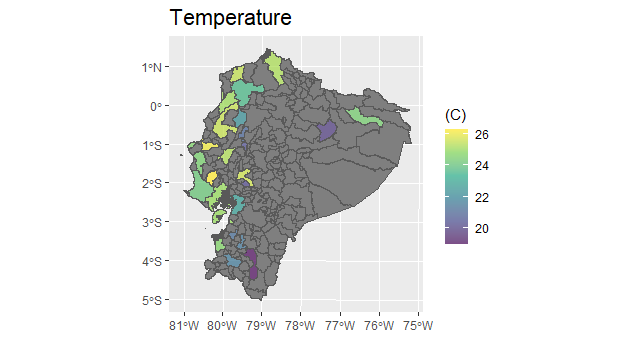
\includegraphics{Rplot.png}
    \caption{Caption}
    \label{fig:enter-label}
\end{figure}


\begin{Schunk}
\begin{Sinput}
> summary(cars)
\end{Sinput}
\begin{Soutput}
     speed           dist       
 Min.   : 4.0   Min.   :  2.00  
 1st Qu.:12.0   1st Qu.: 26.00  
 Median :15.0   Median : 36.00  
 Mean   :15.4   Mean   : 42.98  
 3rd Qu.:19.0   3rd Qu.: 56.00  
 Max.   :25.0   Max.   :120.00  
\end{Soutput}
\end{Schunk}

% latex table generated in R 4.1.3 by xtable 1.8-4 package
% Thu Jan 18 16:41:50 2024
\begin{table}[ht]
\centering
\begin{tabular}{rrr}
  \hline
 & speed & dist \\ 
  \hline
1 & 4.00 & 2.00 \\ 
  2 & 4.00 & 10.00 \\ 
  3 & 7.00 & 4.00 \\ 
  4 & 7.00 & 22.00 \\ 
  5 & 8.00 & 16.00 \\ 
  6 & 9.00 & 10.00 \\ 
  7 & 10.00 & 18.00 \\ 
  8 & 10.00 & 26.00 \\ 
  9 & 10.00 & 34.00 \\ 
  10 & 11.00 & 17.00 \\ 
  11 & 11.00 & 28.00 \\ 
  12 & 12.00 & 14.00 \\ 
  13 & 12.00 & 20.00 \\ 
  14 & 12.00 & 24.00 \\ 
  15 & 12.00 & 28.00 \\ 
  16 & 13.00 & 26.00 \\ 
  17 & 13.00 & 34.00 \\ 
  18 & 13.00 & 34.00 \\ 
  19 & 13.00 & 46.00 \\ 
  20 & 14.00 & 26.00 \\ 
  21 & 14.00 & 36.00 \\ 
  22 & 14.00 & 60.00 \\ 
  23 & 14.00 & 80.00 \\ 
  24 & 15.00 & 20.00 \\ 
  25 & 15.00 & 26.00 \\ 
  26 & 15.00 & 54.00 \\ 
  27 & 16.00 & 32.00 \\ 
  28 & 16.00 & 40.00 \\ 
  29 & 17.00 & 32.00 \\ 
  30 & 17.00 & 40.00 \\ 
  31 & 17.00 & 50.00 \\ 
  32 & 18.00 & 42.00 \\ 
  33 & 18.00 & 56.00 \\ 
  34 & 18.00 & 76.00 \\ 
  35 & 18.00 & 84.00 \\ 
  36 & 19.00 & 36.00 \\ 
  37 & 19.00 & 46.00 \\ 
  38 & 19.00 & 68.00 \\ 
  39 & 20.00 & 32.00 \\ 
  40 & 20.00 & 48.00 \\ 
  41 & 20.00 & 52.00 \\ 
  42 & 20.00 & 56.00 \\ 
  43 & 20.00 & 64.00 \\ 
  44 & 22.00 & 66.00 \\ 
  45 & 23.00 & 54.00 \\ 
  46 & 24.00 & 70.00 \\ 
  47 & 24.00 & 92.00 \\ 
  48 & 24.00 & 93.00 \\ 
  49 & 24.00 & 120.00 \\ 
  50 & 25.00 & 85.00 \\ 
   \hline
\end{tabular}
\caption{Hola} 
\end{table}
Hola como $2$ texto  dist

\begin{Schunk}
\begin{Sinput}
> test <- c("testA", "testB", "testC")
> boldtest <- paste0("\\textbf{", test,"}", collapse = " and ")
\end{Sinput}
\end{Schunk}
